Let $\vec{M}$ be the point that divides the two points $\vec{A}=\myvec{1\\0}$ and $\vec{B}=\myvec{2\\3}$ in ratio $1:n.$
\begin{align}
    \vec{M}=\frac{n\vec{A}+\vec{B}}{n+1}=\frac{n\myvec{1\\0}+\myvec{2\\3}}{n+1}\\
    \implies\vec{M}=\frac{1}{n+1}\myvec{n+2\\3}\nonumber
\end{align}
The direction vector of line AB is
\begin{align}
    \myvec{1\\0}-\myvec{2\\3}=\myvec{-1\\-3}
\end{align}
The direction vector of line AB is normal vector of perpendicular line. Then
\begin{align}
    \vec{n}=\myvec{-1\\-3}
\end{align}
The equation of line in terms of normal vector is then obtained as
\begin{align}
    \vec{n}^T(\vec{x}-\vec{M})&=0\\
    \implies\myvec{-1&-3}&\brak{\vec{x}-\frac{1}{n+1}\myvec{n+2\\3}} = 0\\
    \therefore \myvec{-1&-3}\vec{x}&= \frac{-n-11}{n+1}
\end{align}
We got equation of the line perpendicular to line segment joining points $\vec{A}$ and $\vec{B}$ and dividing them in the ratio $1:n$. 

For plotting let us take $n = 2$, Then the perpendicular line equation will be as,
\begin{align}
    \myvec{-1&-3}\vec{x}&= \frac{-13}{3}
\end{align}
See Fig.     \ref{aug/2/17/1}
\begin{figure}[htp]
    \centering
    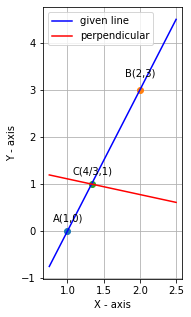
\includegraphics[width=\columnwidth]{solutions/aug/2/17/a_4.png}
    \caption{graphical interpretation}
    \label{aug/2/17/1}
\end{figure}
